\section*{Introduction}
Drug addiction is often treated in a rehabilitation clinic, and relapse occurs
when the patient returns to the original context of their drug use (Higgins,
Budney, \& Bickel, 1995). How can we engineer treatments that generalize between
contexts? Our earlier work \cite{crossley_erasing_2013} showed that
``feedback contingency'' --- used here to indicate the degree of randomness
between response and outcome --- may play a pivotal role in answering this
question.

Crossley et al. (2013) studied procedural modification in a procedural category-learning task. These experiments contained three phases of equal duration:
acquisition, intervention, and test. Participants were trained on the category
structure shown in panel C of Figure \ref{fig:test_cats} during the acquisition
phase. During the intervention phase, the underlying category structure was not
changed, but feedback was manipulated (described in the next paragraph) in an
attempt to erase the learning that occurred during the acquisition phase. During
the test phase, feedback was returned to 100\% veridical (as was the case during
acquisition). Participants in the Relearning condition were tested on the
original acquisition category-response mappings, whereas participants in the New-Learning condition were tested on a permuted category-response mapping. If the original
acquisition-phase learning was preserved through intervention, then test phase
performance in the Relearning condition should be better than acquisition-phase
performance (i.e., participants should show savings), and test-phase performance
in the New-Learning condition should be worse than acquisition-phase performance
(due to interference from initial learning).

\begin{figure}[t]
  \centering 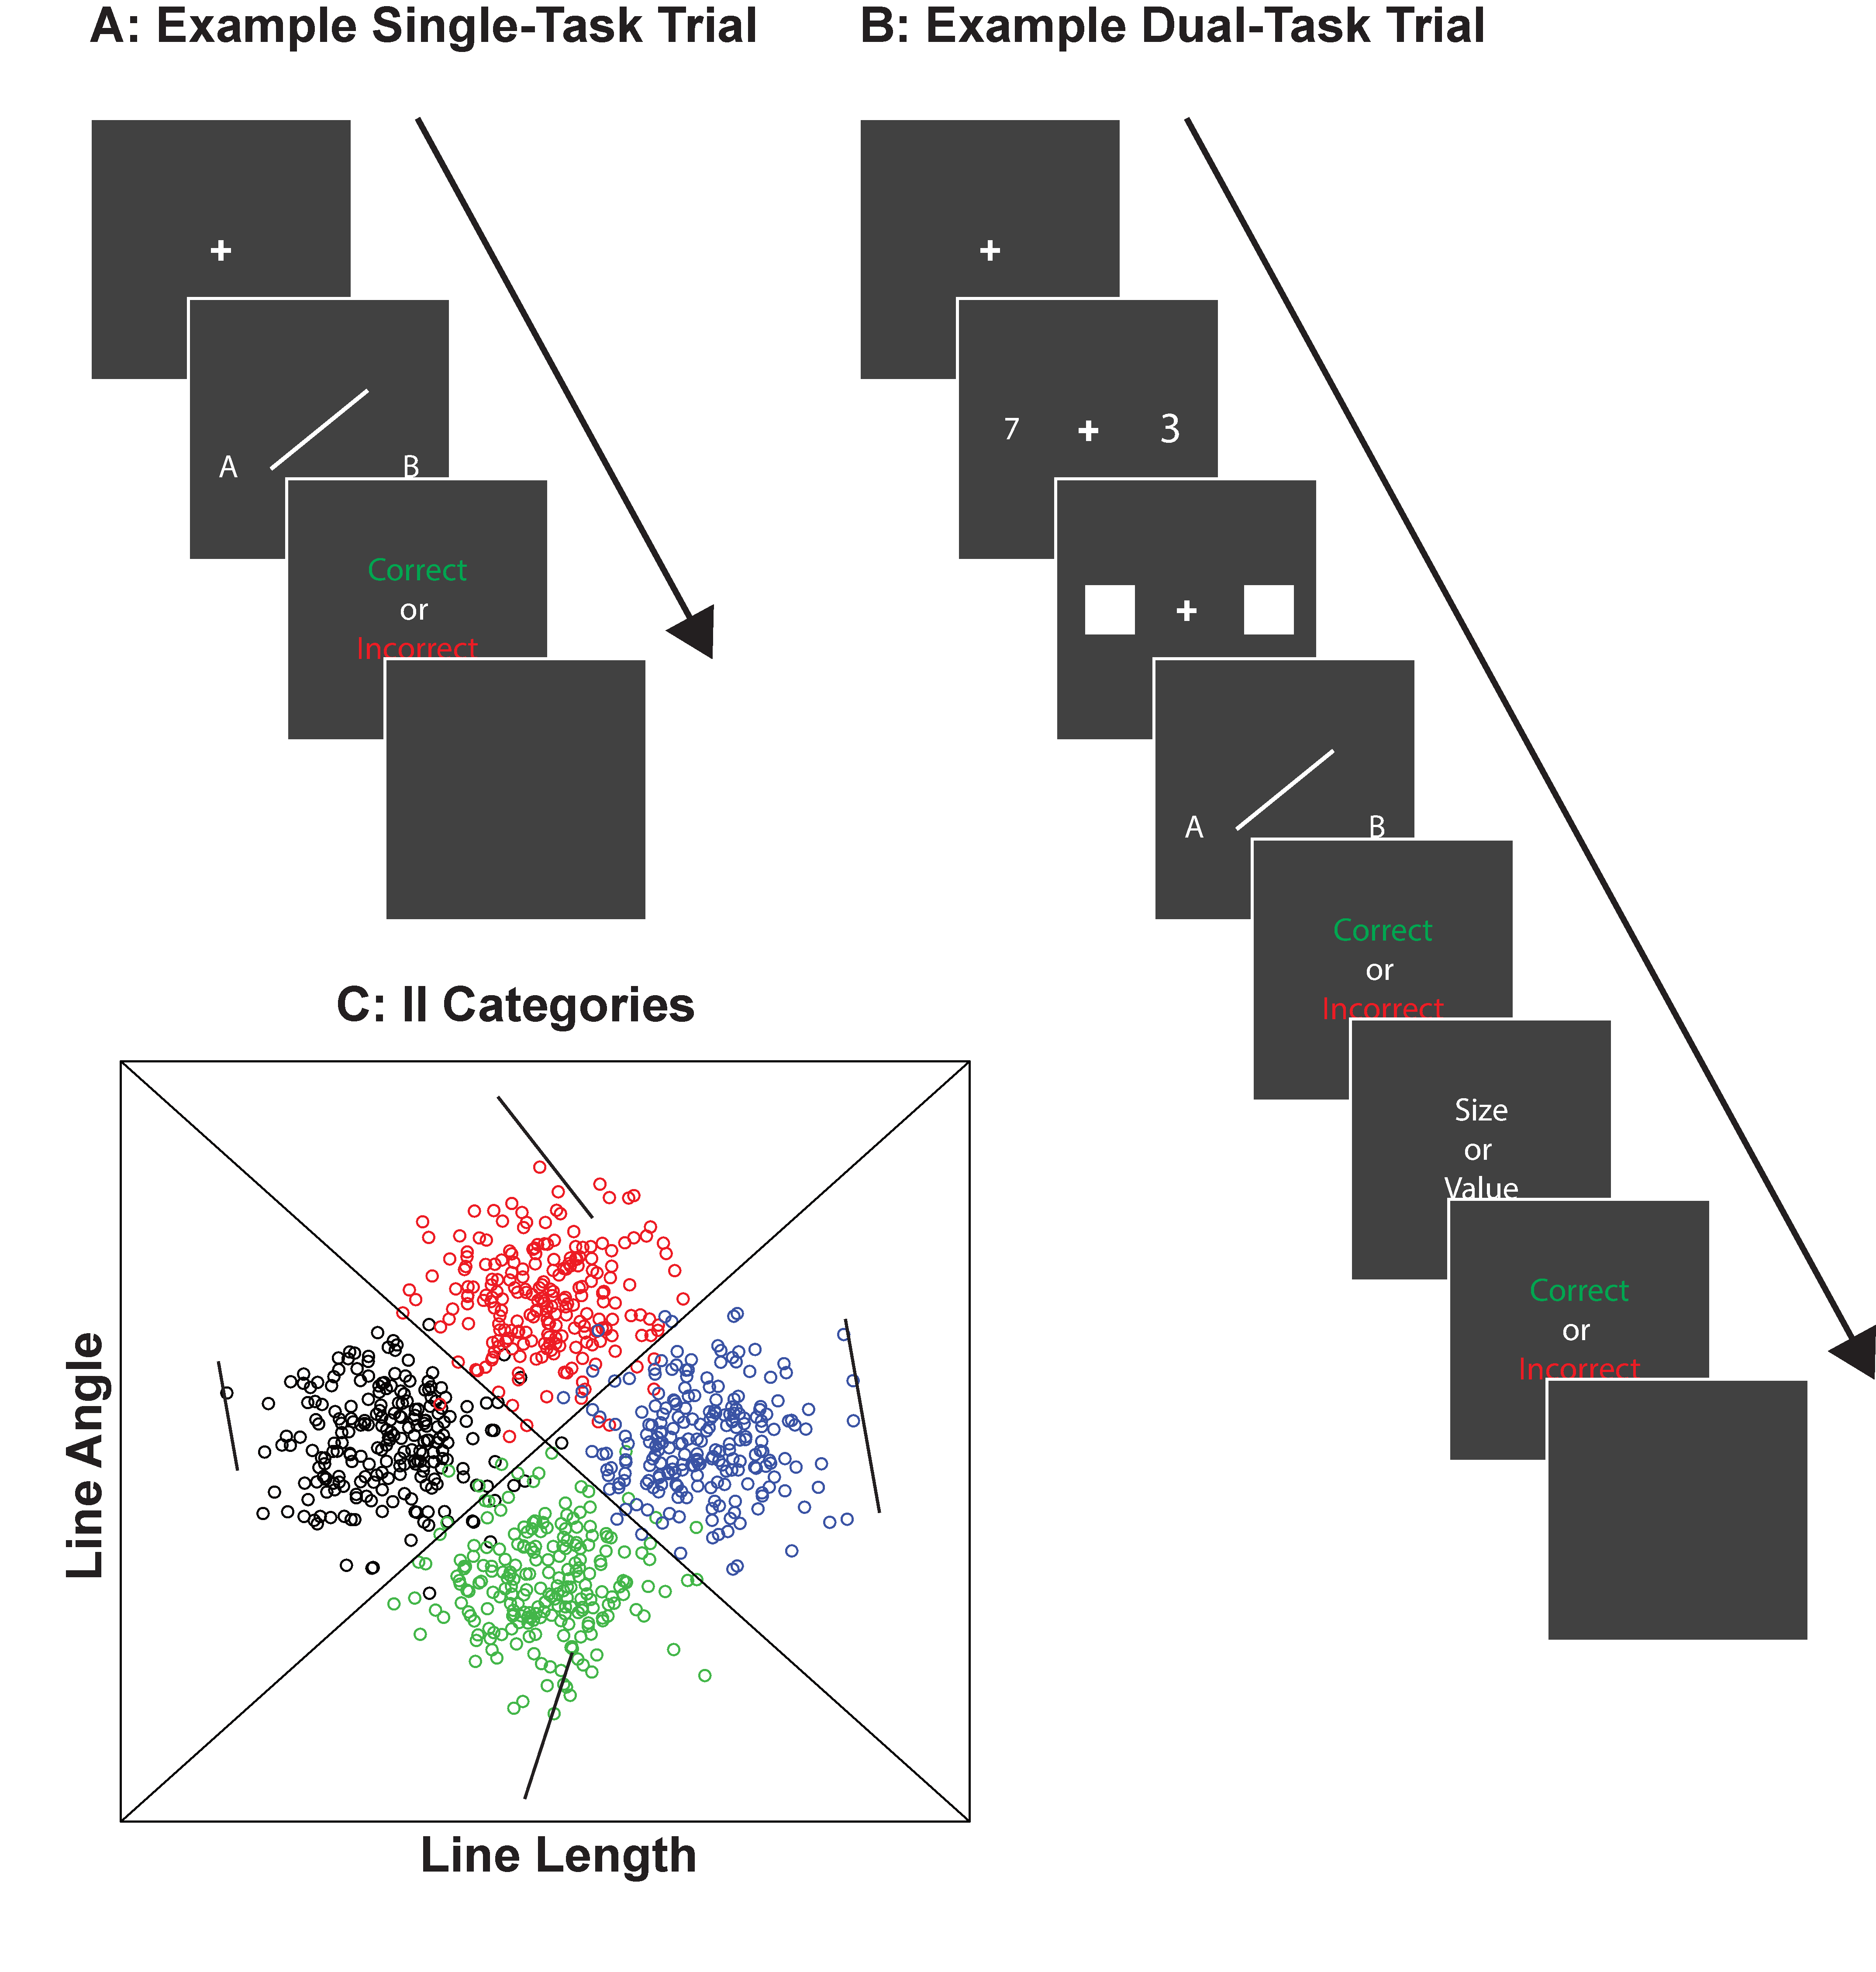
\includegraphics[width=1.0\textwidth]{../figures/fig_trials.pdf}
  \caption{
    \textbf{A:} An Example trial during single-task conditions.
    \textbf{B:} An example trial during dual-task conditions.
    \textbf{C:} The II categories used during the acquisition phase of
    Crossley et al. (2013).
  }
  \label{fig:test_cats}
\end{figure}

The changes in feedback used during the intervention phase were chosen by
considering classic models of procedural learning (panel A of Figure
\ref{fig:models}), which extend classic models of associative learning.
These models assume that procedural knowledge is learned at cortical-striatal
synapses via DA-dependent synaptic plasticity. Consistent with the classic view
that procedural knowledge is robust against forgetting, simply removing feedback
during intervention did not cause any substantial performance change (data not
shown). Therefore, an intervention phase with completely random feedback was
used (i.e., correct feedback was randomly given 25\% of the time). Classic
models predict that this intervention will replace initially acquired S-R
associations with random strengths, thereby leading to identical or attenuated
performance during the test phase in both the Relearning and the New-Learning
conditions. Contrary to this prediction, random-feedback did not disrupt category knowledge. During the test phase, performance relative to initial acquisition was enhanced in the Relearning condition, and attenuated in the New-Learning condition; both suggesting savings
(left panel of Figure \ref{fig:unlearning_data}).

\begin{figure}[h]
  \centering 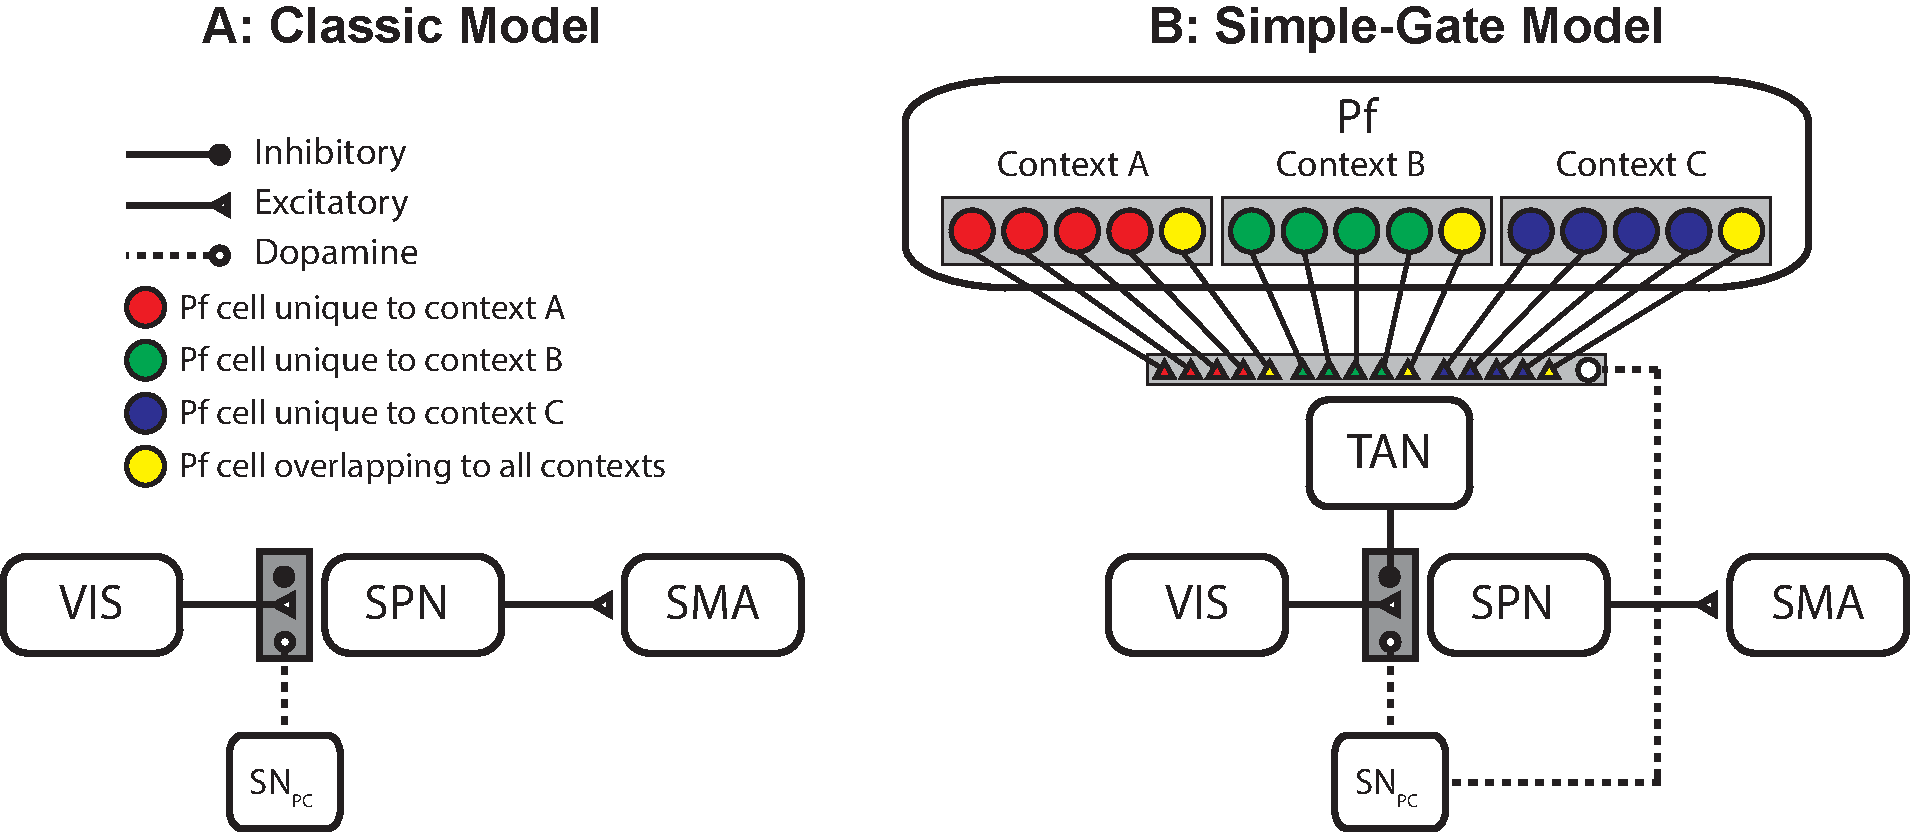
\includegraphics[width=1.0\textwidth]{../figures/fig_models.pdf}
  \caption{ \textbf{A: The Classic Model.} A classic model of procedural
    learning based on a greatly simplified representation of the ``direct pathway''
    through the basal ganglia. S-R associations are learned at cortical-striatal
    synapses, which are modified via dopamine-dependent reinforcement learning. The
    likelihood of repeating actions that lead to \emph{unexpected} positive outcomes
    is gradually increased, and the likelihood of repeating actions that lead to
    \emph{unexpected} negative outcomes is gradually decreased. \textbf{B: The
      TANs Model.} The classic model of procedural learning with the
    addition of a context-specific Pf-TAN pathway. This pathway acts as a gate on
    cortical-striatal synaptic plasticity, permitting or preventing the learning and
    expression of procedural knowledge. (MSN - medium spiny neuron of the striatum. D1 -
    Direct pathway MSN expressing the D1 DA receptor. D2 - Indirect pathway MSN
    expressing the D2 DA receptor. SMA - Supplementary Motor Area. SNpc - substantia
    nigra pars compacta. Pf - parafascicular nucleus of the thalamus. VIS - visual
    cortex)}
  \label{fig:models}
\end{figure}

The random feedback intervention result implies that \textit{there is a gating
mechanism that protects procedural learning from modification during random
feedback.} One candidate biological system for this gating mechanism is the
striatal cholinergic interneurons called TANs (for Tonically Active Neurons). It
is thought that these neurons mediate cortical-striatal synaptic plasticity via
presynaptic inhibition of cortical inputs to the striatum (Figure
\ref{fig:models}). As their name suggests, the TANs are tonically active in
their default state; however, they learn to pause their firing when stimuli that
predict reward are encountered. This allows striatal neurons to respond to
cortical input, and cortical-striatal learning to take place. The TANs are driven
by the parafascicular (Pf) nucleus in the thalamus, which signals salient
environmental cues; their pause response occurs only when the Pf-TAN synapse is
strong. The learning at both Pf-TAN synapses and cortical-striatal synapses
is driven by the DA reinforcement signal.

An updated procedural learning model that includes the TAN gating mechanism has
been shown to account for a variety of behavioral and physiological data from
simple instrumental conditioning tasks
\cite{ashby_computational_2011, crossley_expanding_2016}, including rapid
relearning following extinction. However, the model fails to account for the
random feedback results described above. This failure stems from the way DA
activity is modeled. In the model, DA firing reflects a reward prediction error
(RPE; which equals the difference between the obtained and expected outcome), and since
random feedback is \emph{by definition} completely unpredictable, it leads to
persistent RPEs and corresponding DA fluctuations during random feedback. These
fluctuations prevent the TANs from closing the gate on cortical-striatal
plasticity, and thereby permit random feedback to disrupt initial learning.

In order for the TANs to reliably close the gate and protect cortical-striatal
plasticity during random feedback, two conditions must be met:

\begin{description}
\item \textit{1. The model must detect when feedback has become random.} Random
  feedback has several properties, but our results suggest that the most critical -- at least with respect to learning and unlearning -- is that random feedback is non-contingent on action. More specifically, when the feedback is random the correlation between response confidence and feedback valence is zero. This correlation, which we refer to as \textit{feedback contingency}, is a critical requirement of successful learning. For example, \citeA{AshbyVucovich2016} compared learning under high and low levels of feedback contingency in two different category-learning tasks -- one that recruits declarative memory and one that recruits procedural memory. In both tasks, the high- and low-contingency conditions used exactly the same stimuli, had exactly the same optimal strategies, and optimal accuracy was 80\% correct in all conditions. The results were virtually identical in the two tasks. Learning was good when feedback contingency was high, but degrading feedback contingency seemed to abolish all learning in most participants.

\item \textit{2. The TANs must close the gate when non-contingent (e.g., random) feedback is detected.} This only occurs when Pf-TAN synapses undergo consistent weakening. This was modeled in \cite{crossley_erasing_2013} by assuming that the magnitude of \textit{the DA response is attenuated and biased below baseline when feedback contingency is low.}
\end{description}

With this modification to the DA system, the model not only accounts for savings
in relearning after random feedback intervention, but also makes a novel
prediction: \textit{Mixed feedback that contains some random and some veridical feedback trials produces an intermediate level of contingency and therefore should prevent the TANs from completely closing the gate on cortical-striatal plasticity, thereby enabling modification of initial learning.} Our results supported this prediction (panel B of Figure \ref{fig:unlearning_data}) -- that is, performance during the Test phase was identical in the Relearning and New-Learning conditions, and each was significantly different from initial learning.

One potential confound of this mixed-feedback intervention was that the rate of positive feedback was greater than during the random-feedback intervention
(note the different accuracy levels during the intervention phase in panels A
and B of Figure \ref{fig:unlearning_data}). To address this confound, Crossley
et al. (2013) examined performance with an intervention that included random
feedback, but with a positive feedback rate of 40\%. This intervention increased the
overall positive feedback rate, but since it was entirely random, feedback
contingency was still zero. The results from this experiment are shown in panel
C of Figure \ref{fig:unlearning_data}, and are virtually identical to our original random feedback intervention (where the positive feedback rate was 25\%, see panel A,
Figure \ref{fig:unlearning_data}). Thus, mixed feedback intervention may
constitute an effective intervention for procedural modification.

\begin{figure}[h]
  \centering 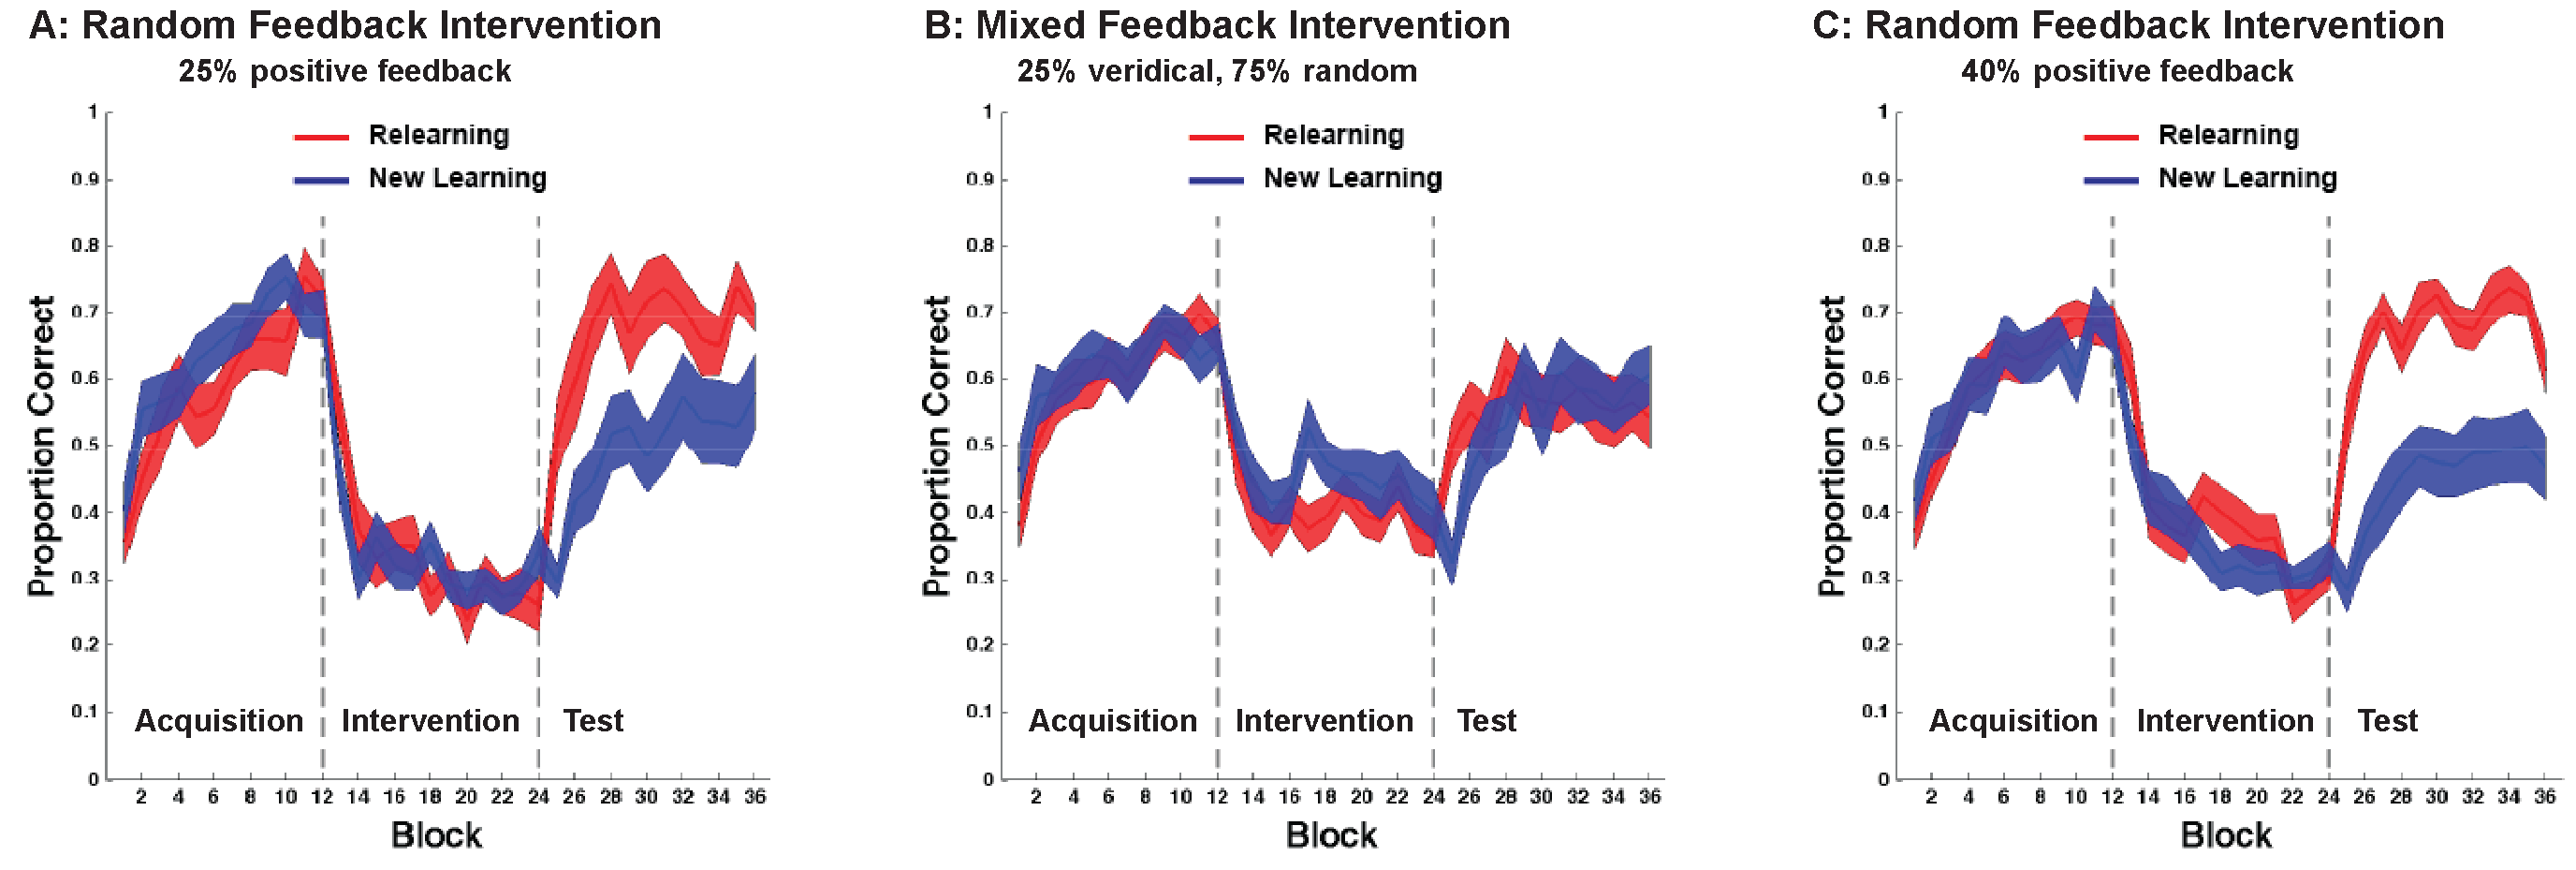
\includegraphics[width=1.0\textwidth]{../figures/fig_unlearning_results.pdf}
  \caption{
    Behavioral results with different interventions. \textbf{A:} Random
    feedback intervention with 25\% positive feedback. Accuracy drops to near chance
    during intervention, but is reacquired faster than original learning in the
    Relearning condition (red). In contrast, a lasting interference is observed in
    the New Learning condition (blue). Both results are consistent with the
    hypothesis that initial learning was not overwritten by random feedback.
    \textbf{B:} Mixed feedback intervention. Accuracy drops during intervention --
    though not to chance (i.e., 25\%) -- but subsequent learning proceeds at
    approximately the same rate and to the same extent as initial learning when
    either the original category-response mappings (red) or new category-response
    mappings (blue) are introduced. These results are consistent with the hypothesis
    that initial learning was overwritten during the intervention. \textbf{C:}
    Random feedback intervention with 40\% positive feedback. Results are
    qualitatively identical to random feedback intervention with 25\% positive
    feedback, implying that the mixed feedback results were driven by feedback
    contingency and not by positive feedback. }
  \label{fig:unlearning_data}
\end{figure}

Crossley et al. (2013) hypothesized that the gate on procedural learning --- and
therefore the key to procedural modification --- is controlled by the degree of
feedback contingency. Even so, we made no predictions about how contingency is computed by the nervous system. This article begins addressing this question -- by asking whether feedback contingency is computed via declarative mechanisms (e.g., prefrontal networks involved in working memory and executive reasoning). Our rationale is as follows: If feedback contingency is estimated by declarative mechanisms, then increasing cognitive load during the intervention phase (by requiring participants to simultaneously perform a dual task) should impair the ability of participants to detect a change to random feedback, which should cause the TANs gate to remain open, thereby allowing random feedback to modify the procedural knowledge that was acquired during initial learning. 

With this goal in mind, we performed an experiment that mimicked the design of Crossley et al. (2013), except we added a concurrent numerical Stroop task during key classification trials. Previous research suggests that this dual task interferes with category learning that recruits declarative memory but not with category learning that recruits procedural memory \cite{WaldronAshby2001}. Thus, since our categorization task recruits procedural memory, any effect of the dual task on categorization performance should be due to its effects on contingency estimation, rather than on category learning per se.

In conditions 1 -- 3, the first dual-task trial was 50 trials before the onset of intervention, and continued for 100, 200, or 300 trials, respectively. In Condition 4, the first dual-task trial was 50 trials after the onset of intervention, and continued for 250 trials.
Comparing conditions 1 -- 3 to condition 4 will allow us to assess the
importance of disrupting the estimation of feedback contingency during the 
transition from acquisition to intervention. Condition 5 was a control condition
in which no concurrent Stroop task was ever performed. 

If feedback contingency estimation depends on declarative mechanisms then
two behavioral markers are expected: (1) the dual task should slow the drop in categorization accuracy that occurs with the onset of random feedback; and (2) reacquisition of the original category learning should be slower in the dual task conditions than in the no dual-task control.